% TikZ in a cmyk-option document: fills, strokes, text and named colours all through xcolor.
\documentclass{article}
\usepackage[cmyk]{xcolor}
\usepackage{tikz}
\pagestyle{empty}
\begin{document}
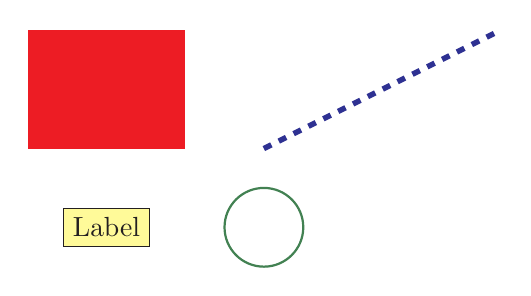
\begin{tikzpicture}
  \fill[red] (0,0) rectangle (2,1.5);
  \draw[line width=2pt,blue,dashed] (3,0) -- (6,1.5);
  \node[draw=black,fill=yellow!40,text=black] at (1,-1) {Label};
  \draw[green!60!black,thick] (3,-1) circle (0.5);
\end{tikzpicture}
\end{document}
